\documentclass[11pt]{article}

% ---------------------------------------------------------------------------
%  Spatial-domain mapping of human cortex -- SRI Research Proposal
%  Compile with:  tectonic docs/proposal.tex
% ---------------------------------------------------------------------------

\usepackage[margin=1in]{geometry}
\usepackage{amsmath,amssymb}
\usepackage{xcolor}
\usepackage{tikz}
\usetikzlibrary{arrows.meta,positioning,fit,backgrounds,calc,shapes.geometric}
\usepackage{booktabs}
\usepackage{array}
\usepackage{colortbl}
\usepackage[most]{tcolorbox}
\usepackage{enumitem}
\usepackage{graphicx}
\usepackage[colorlinks=true,linkcolor=sriblue,citecolor=sriblue,urlcolor=sriaccent]{hyperref}

% ----- Palette -------------------------------------------------------------
\definecolor{sriblue}{HTML}{1F4E79}
\definecolor{sriaccent}{HTML}{E8684A}
\definecolor{srigreen}{HTML}{2E8B57}
\definecolor{srigray}{HTML}{4B5563}
\definecolor{srilight}{HTML}{EAF1F8}
\definecolor{sriamber}{HTML}{F6BD16}
\definecolor{srirow}{HTML}{F2F6FB}
\definecolor{srired}{HTML}{C0392B}
\definecolor{domA}{HTML}{E8684A}
\definecolor{domB}{HTML}{5B8FF9}
\definecolor{domC}{HTML}{2E8B57}

\usepackage{titlesec}
\titleformat{\section}{\large\bfseries\color{sriblue}}{\thesection}{0.6em}{}
\titleformat{\subsection}{\normalsize\bfseries\color{sriblue!85!black}}{\thesubsection}{0.5em}{}
\titlespacing*{\section}{0pt}{1.4ex}{0.8ex}

\newtcolorbox{problembox}{colback=srilight,colframe=sriblue,boxrule=0.9pt,
  arc=2pt,left=6pt,right=6pt,top=5pt,bottom=5pt}
\newtcolorbox{gapbox}{colback=sriaccent!8,colframe=sriaccent,boxrule=0.9pt,
  arc=2pt,left=6pt,right=6pt,top=5pt,bottom=5pt}
\newtcolorbox{aimbox}[1]{colback=srigreen!7,colframe=srigreen,boxrule=0.8pt,
  arc=2pt,left=6pt,right=6pt,top=4pt,bottom=4pt,title={#1},
  fonttitle=\bfseries\color{white},colbacktitle=srigreen}

\renewcommand{\arraystretch}{1.25}
\newcommand{\NN}{\mathcal{N}}

\begin{document}

\begin{center}
  {\LARGE\bfseries\color{sriblue} Localizing Molecular Pathology in the\\ Human Cerebral Cortex}\\[3pt]
  {\large\bfseries\color{sriblue!80!black} Scalable, layer-resolved tissue mapping from spatial transcriptomics\\ to study neuropsychiatric and neurodegenerative disease}\\[10pt]
  {\large Akshatha Arunkumar}\\[2pt]
  {\small Student Research Institute (SRI) -- Summer 2026 Cohort \\
  Harvard Undergraduate OpenBio Laboratory}\\[2pt]
  {\small\itshape Research Proposal for Mentor Review \quad\textbar\quad \today}
\end{center}

\vspace{2pt}
\begin{problembox}
\textbf{The problem.} The human cerebral cortex is organized into six cellular
layers whose disruption underlies disorders from schizophrenia to Alzheimer's
disease. New spatial-transcriptomics technologies can finally measure gene
expression \emph{while preserving each cell's location}, opening the door to
asking \emph{where} in the tissue molecular pathology begins. But to do so we
must first assign every measured spot to its correct cortical layer -- a step
that today is done by slow, subjective manual annotation and does not scale to
the many tissue sections a disease study requires. This project develops an
accurate, automated, label-efficient method for that mapping step.
\end{problembox}

\begin{aimbox}{Preliminary result -- already obtained on real human cortex}
On the gold-standard LIBD DLPFC benchmark (12 Visium sections, 47{,}329
expert-annotated spots, 7 cortical domains), a pilot of the proposed spatial GNN
reaches \textbf{macro-F1 $0.755$ / ARI $0.654$} under cross-section evaluation
(whole tissues held out, 3 seeds), versus \textbf{XGBoost $0.516$ / $0.369$} and
\textbf{MLP $0.484$ / $0.375$} on identical expression features -- a $+0.24$
macro-F1 win. A graph-removal ablation collapses the identical GNN back onto the
blind MLP (F1 $0.49$), confirming the advantage is \emph{spatial}, not features.
The win is \textbf{architecture-robust} (a graph-attention GAT encoder matches
GraphSAGE at $\sim$$0.75$ F1) and \textbf{generalizes to a second technology}: on
single-cell \emph{osmFISH} mouse cortex (33 genes, true region labels) the GNN
reaches \textbf{macro-F1 $0.96$} versus $0.54$ (XGBoost) and $0.63$ (MLP). The
proposal below formalizes, stress-tests, and extends these results.
\end{aimbox}

% ===========================================================================
\section{Background and Significance}

The cerebral cortex is a layered structure: six neuronal laminae (L1--L6) above
the white matter, each with a distinct composition of cell types and gene
expression. This laminar architecture is not incidental -- it organizes cortical
computation, and its disruption is a recurring theme in disease:

\begin{itemize}[leftmargin=1.4em,itemsep=1pt]
\item \textbf{Schizophrenia:} layer-specific deficits in interneurons and
pyramidal-neuron signalling in the dorsolateral prefrontal cortex (DLPFC).
\item \textbf{Alzheimer's disease:} neurofibrillary tau pathology follows a
\emph{laminar} distribution, with specific layers selectively vulnerable.
\item \textbf{Autism spectrum disorder:} abnormalities of cortical lamination
and minicolumnar organization.
\end{itemize}

Because these changes are \emph{spatially localized}, understanding them
requires methods that respect tissue location. Spatial transcriptomics (10x
Visium, MERFISH, Xenium) now provides exactly this -- genome-wide expression at
thousands of spatially-registered spots per tissue section. The scientific
prize is the ability to pinpoint \emph{which layer}, and \emph{which molecular
programs within it}, change in disease.

\begin{table}[h]
\centering\small
\begin{tabular}{>{\raggedright\arraybackslash}p{0.30\linewidth} >{\raggedright\arraybackslash}p{0.62\linewidth}}
\toprule
\rowcolor{sriblue}\color{white}\textbf{Why it matters} & \color{white}\textbf{Consequence}\\
\midrule
\rowcolor{srirow} Cortical function is layer-organized & Disease changes are layer-specific, not diffuse.\\
Spatial omics preserves location & We can finally ask \emph{where} pathology starts.\\
\rowcolor{srirow} But spots must be assigned to layers first & Domain mapping is the rate-limiting step for every downstream analysis.\\
\bottomrule
\end{tabular}
\caption{Accurate spatial-domain mapping is the enabling step that turns spatial
transcriptomics into layer-resolved disease biology.}
\label{tab:significance}
\end{table}

% ===========================================================================
\section{The Unmet Need}

To attribute a molecular change to a cortical layer, every spot must first be
labelled with its domain. Today this is done in two unsatisfactory ways:

\begin{gapbox}
\textbf{Gap 1 -- Manual annotation does not scale.} Expert layer annotation of a
single section is slow and subjective; disease cohorts require dozens of
sections across many donors, where manual labelling becomes the bottleneck.\\[3pt]
\textbf{Gap 2 -- Non-spatial analysis fragments tissue.} Clustering spots by
expression alone ignores location, producing spatially incoherent, noisy domains
because a single spot's expression is sparse and dropout-corrupted.
\end{gapbox}

\noindent What is needed is an \emph{automated} method that is \emph{accurate},
\emph{label-efficient} (learns from a few annotated sections and transfers to
new ones), and \emph{spatially coherent}. The central scientific observation we
exploit is simple: \textbf{a spot's layer is a property of its spatial
neighbourhood} -- adjacent spots overwhelmingly share a layer -- so the
information missing from one noisy spot is present in the tissue around it
(Fig.~\ref{fig:mechanism}).

\begin{figure}[h]
\centering
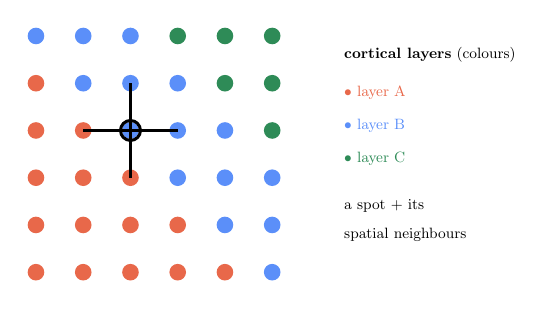
\begin{tikzpicture}[scale=0.6,every node/.style={transform shape}]
  \foreach \i in {0,...,5}{
    \foreach \j in {0,...,5}{
      \pgfmathtruncatemacro{\sum}{\i+\j}
      \ifnum\sum<5
        \definecolor{cc}{HTML}{E8684A}
      \else
        \ifnum\sum<8 \definecolor{cc}{HTML}{5B8FF9}\else\definecolor{cc}{HTML}{2E8B57}\fi
      \fi
      \node[circle,fill=cc,minimum size=10pt,inner sep=0pt] (n\i\j) at (\i,\j) {};
    }
  }
  \node[circle,draw=black,line width=1.1pt,minimum size=12pt,inner sep=0pt] at (2,3) {};
  \foreach \a/\b in {1/3,3/3,2/2,2/4}{\draw[black,line width=1pt] (2,3)--(\a,\b);}
  \node[anchor=west,font=\small] at (6.4,4.6) {\textbf{cortical layers} (colours)};
  \node[anchor=west,font=\small,domA] at (6.4,3.8) {$\bullet$ layer A};
  \node[anchor=west,font=\small,domB] at (6.4,3.1) {$\bullet$ layer B};
  \node[anchor=west,font=\small,domC] at (6.4,2.4) {$\bullet$ layer C};
  \node[anchor=west,font=\small] at (6.4,1.4) {a spot + its};
  \node[anchor=west,font=\small] at (6.4,0.8) {spatial neighbours};
\end{tikzpicture}
\caption{Layers are spatially contiguous, so a spot's label agrees with its
neighbours'. A single (noisy) spot may be ambiguous, but its neighbourhood
reveals its layer -- the signal an analysis must use.}
\label{fig:mechanism}
\end{figure}

% ===========================================================================
\section{Research Aims}

\begin{aimbox}{Aims}
\textbf{Aim 1.} Develop an automated method that maps spatial-transcriptomics
spots to cortical layers accurately and label-efficiently.\\
\textbf{Aim 2.} Show it \emph{transfers across tissue sections} (train on some,
predict on new ones), the regime that matters for disease cohorts.\\
\textbf{Aim 3.} Verify the result is biologically grounded -- recover known
layer marker genes and surface candidate annotation errors for expert review.
\end{aimbox}

\noindent\textbf{Guiding questions.} (Q1) Can layer identity be predicted
accurately from spatial transcriptomics? (Q2) Does explicitly modelling tissue
\emph{neighbourhood} improve accuracy over analysing each spot in isolation, and
by how much? (Q3) Do the predictions recover known cortical-layer biology?

% ===========================================================================
\section{Data}

\begin{table}[h]
\centering\small
\begin{tabular}{>{\raggedright\arraybackslash}p{0.26\linewidth} >{\raggedright\arraybackslash}p{0.40\linewidth} >{\raggedright\arraybackslash}p{0.26\linewidth}}
\toprule
\rowcolor{sriblue}\color{white}\textbf{Resource} & \color{white}\textbf{Content} & \color{white}\textbf{Role}\\
\midrule
\rowcolor{srirow} LIBD DLPFC (10x Visium) & 12 sections, $\sim$48k spots, expert manual layer annotations (L1--L6 + WM) & Real ground-truth benchmark\\
Controlled synthetic tissue & layers defined by neighbourhood; per-spot signal deliberately noisy & Method validation / ablation\\
\rowcolor{srirow} osmFISH mouse cortex & single-cell resolution, 33 genes, $\sim$4.8k cells, region labels & Second-technology generalization\\
\bottomrule
\end{tabular}
\caption{All data are public and de-identified post-mortem tissue. The LIBD
DLPFC dataset is the field-standard ground truth for cortical-layer mapping.}
\label{tab:data}
\end{table}

% ===========================================================================
\section{Proposed Methodology}

The neighbourhood structure in Fig.~\ref{fig:mechanism} motivates representing
each tissue section as a \textbf{spatial graph}: nodes are spots, edges connect
each spot to its $k$ nearest spatial neighbours, and node features are the spot's
(preprocessed) gene expression. Crucially, \emph{coordinates are used only to
build the graph, never as features}, so any benefit is attributable to using
tissue structure rather than memorizing absolute position.

\subsection{Proposed model: a spatial graph neural network}
We propose a graph neural network (GNN) that classifies each spot's layer by
pooling information across its spatial neighbourhood. With a GraphSAGE encoder
over $L$ layers of message passing,
\begin{equation}
h_v^{(l)} = \sigma\!\Big( W^{(l)}\big[\,h_v^{(l-1)} \,\big\Vert\,
\textstyle\operatorname*{AGG}_{u\in\NN(v)} h_u^{(l-1)}\,\big]\Big),
\qquad \hat{y}_v = \operatorname{softmax}\!\big(W_o\, h_v^{(L)}\big),
\label{eq:sage}
\end{equation}
trained with cross-entropy on annotated spots. The aggregation step pools the
neighbourhood, denoising the sparse per-spot signal -- exactly the property
Gap~2 lacks. We will compare GraphSAGE, GCN, and graph-attention variants.

\begin{figure}[h]
\centering
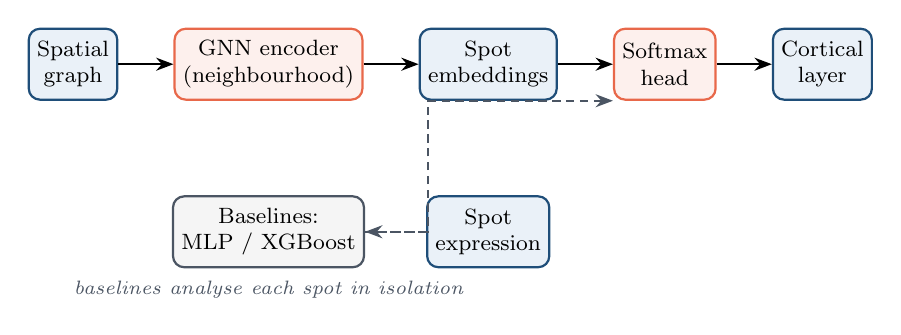
\begin{tikzpicture}[
  node distance=6mm and 7mm,
  box/.style={rounded corners,draw=sriblue,fill=srilight,thick,minimum height=0.9cm,align=center,font=\footnotesize,inner sep=3pt},
  red/.style={rounded corners,draw=sriaccent,fill=sriaccent!10,thick,minimum height=0.9cm,align=center,font=\footnotesize,inner sep=3pt},
  gray/.style={rounded corners,draw=srigray,fill=gray!8,thick,minimum height=0.9cm,align=center,font=\footnotesize,inner sep=3pt},
  >={Stealth[length=2.2mm]}]
  \node[box] (g) {Spatial\\graph};
  \node[red,right=of g] (enc) {GNN encoder\\(neighbourhood)};
  \node[box,right=of enc] (z) {Spot\\embeddings};
  \node[red,right=of z] (dec) {Softmax\\head};
  \node[box,right=of dec] (s) {Cortical\\layer};
  \draw[->,thick] (g)--(enc); \draw[->,thick] (enc)--(z);
  \draw[->,thick] (z)--(dec); \draw[->,thick] (dec)--(s);
  \node[gray,below=12mm of enc] (mlp) {Baselines:\\MLP / XGBoost};
  \node[box,below=12mm of z] (xf) {Spot\\expression};
  \draw[->,thick,densely dashed,srigray] (xf)--(mlp);
  \draw[->,thick,densely dashed,srigray] (mlp.east) -- ++(0.8,0) |- (dec.south west);
  \node[srigray,font=\scriptsize\itshape,below=1pt of mlp] {baselines analyse each spot in isolation};
\end{tikzpicture}
\caption{Proposed pipeline. The GNN (orange) pools each spot's spatial
neighbourhood; the non-spatial baselines (gray) classify each spot alone.}
\label{fig:pipeline}
\end{figure}

\subsection{Baselines and rigorous evaluation}
We benchmark the GNN against strong non-spatial models on the \emph{same}
expression features, so the comparison isolates the value of using tissue
structure.

\begin{table}[h]
\centering\small
\begin{tabular}{>{\raggedright\arraybackslash}p{0.20\linewidth} >{\raggedright\arraybackslash}p{0.28\linewidth} >{\raggedright\arraybackslash}p{0.44\linewidth}}
\toprule
\rowcolor{sriblue}\color{white}\textbf{Model} & \color{white}\textbf{Uses tissue structure?} & \color{white}\textbf{Purpose}\\
\midrule
\rowcolor{srirow} \textbf{Spatial GNN (proposed)} & yes (neighbourhood) & layer mapping that respects tissue\\
XGBoost & no & strong tabular baseline on expression\\
\rowcolor{srirow} MLP & no (features only) & structure-blind control\\
\bottomrule
\end{tabular}
\caption{Baselines use the same per-spot expression features the GNN starts
from; only the GNN sees the spatial graph.}
\label{tab:models}
\end{table}

\noindent\textbf{Leakage-safe splits.} (i) \emph{Cross-section} -- whole
sections are held out for testing; since layer layouts differ per section,
position cannot transfer and only neighbourhood-relative reasoning generalizes
(the disease-cohort regime). (ii) \emph{Within-section} -- contiguous spatial
blocks are held out. \textbf{Metrics:} accuracy, macro-F1 (layers are
imbalanced), and the adjusted Rand index (ARI, the field-standard domain
metric), as mean$\pm$std over 5 seeds.

% ===========================================================================
\section{Rigor: Ablations and Biological Interpretation}

\subsection{Is the spatial structure really doing the work? (falsification)}
We run the identical GNN on three graphs; if the gain is genuinely spatial,
destroying tissue structure must erase it.

\begin{table}[h]
\centering\small
\begin{tabular}{>{\raggedright\arraybackslash}p{0.22\linewidth} >{\raggedright\arraybackslash}p{0.50\linewidth} >{\raggedright\arraybackslash}p{0.20\linewidth}}
\toprule
\rowcolor{sriblue}\color{white}\textbf{Condition} & \color{white}\textbf{Graph given to the model} & \color{white}\textbf{Expected}\\
\midrule
\rowcolor{srirow} Intact & true spatial $k$NN graph & high\\
Shuffled & random edges, same count & $\approx$ baseline\\
\rowcolor{srirow} Empty & no edges & $\approx$ baseline\\
\bottomrule
\end{tabular}
\caption{The ablation makes the central claim falsifiable.}
\label{tab:ablation}
\end{table}

\subsection{Biological interpretation $\rightarrow$ discovery}
For each predicted layer we will (i) extract the genes driving predictions and
confirm recovery of \textbf{known cortical-layer marker genes} used in manual
annotation, and (ii) flag spots where the model confidently disagrees with the
manual label -- candidate \emph{annotation errors} or genuine micro-domains for
expert review. This turns an accuracy metric into biological insight.

% ===========================================================================
\section{Alignment with Strong-Research Criteria}

\begin{table}[h]
\centering\small
\begin{tabular}{>{\raggedright\arraybackslash}p{0.30\linewidth} >{\raggedright\arraybackslash}p{0.62\linewidth}}
\toprule
\rowcolor{sriblue}\color{white}\textbf{Criterion} & \color{white}\textbf{Commitment}\\
\midrule
\rowcolor{srirow} Real, sizable public data & LIBD DLPFC: 12 sections, $\sim$48k annotated spots.\\
Clear medical motivation & Layer-resolved localization of disease pathology.\\
\rowcolor{srirow} Rigorous evaluation & XGBoost + MLP baselines; leakage-safe splits; 5 seeds; macro-F1 + ARI.\\
Interpretability $\rightarrow$ discovery & Recover layer markers; surface candidate annotation errors.\\
\rowcolor{srirow} Ablations & Graph removal, message-passing depth, neighbourhood size.\\
Translational impact & Enables scalable, layer-resolved disease studies.\\
\bottomrule
\end{tabular}
\caption{The project is structured around the elements of strong research.}
\label{tab:formula}
\end{table}

% ===========================================================================
\section{Expected Outcomes}

A proposal states targets, not measured results.

\begin{table}[h]
\centering\small
\begin{tabular}{>{\raggedright\arraybackslash}p{0.26\linewidth} >{\raggedright\arraybackslash}p{0.66\linewidth}}
\toprule
\rowcolor{sriblue}\color{white}\textbf{Outcome} & \color{white}\textbf{Target}\\
\midrule
\rowcolor{srirow} Accurate layer mapping & High macro-F1/ARI on held-out DLPFC sections.\\
Value of tissue structure & Spatial model clearly $>$ non-spatial baselines, with the gap widening across sections.\\
\rowcolor{srirow} Causal check & Graph-removal ablation collapses the spatial model to the baseline.\\
Biological grounding & Recovered layer markers; candidate annotation errors flagged.\\
\rowcolor{srirow} Honesty clause & Any narrowing of the gap is reported as-is; baselines are strong and splits leakage-safe.\\
\bottomrule
\end{tabular}
\caption{Success is a scalable, accurate, biologically-grounded layer-mapping
method validated on real cortex.}
\label{tab:success}
\end{table}

% ===========================================================================
\section{Eight-Week Timeline}

\begin{table}[h]
\centering\small
\begin{tabular}{>{\raggedright\arraybackslash}p{0.14\linewidth} >{\raggedright\arraybackslash}p{0.78\linewidth}}
\toprule
\rowcolor{sriblue}\color{white}\textbf{Weeks} & \color{white}\textbf{Milestones}\\
\midrule
\rowcolor{srirow} 1--2 & Data pipeline (DLPFC to AnnData; spatial-graph builder); synthetic validation tissue.\\
3--4 & Implement proposed spatial model + baselines (XGBoost, MLP); shared trainer.\\
\rowcolor{srirow} 5 & Cross-section + within-section experiments, 5 seeds, macro-F1/ARI.\\
6 & Ablations: graph removal, depth, neighbourhood size.\\
\rowcolor{srirow} 7 & Biological interpretation: layer markers; candidate annotation errors.\\
8 & Figures, tables, manuscript; reproducibility package.\\
\bottomrule
\end{tabular}
\caption{Schedule for the eight-week SRI cohort.}
\label{tab:timeline}
\end{table}

% ===========================================================================
\section{Reproducibility and Ethics}

Implementation uses open tools (PyTorch Geometric for the model; scanpy/anndata
for spatial-omics I/O). All code, configs, seeds, and a data manifest will be
released. No human subjects are involved; all inputs are public, de-identified
post-mortem tissue data. Predictions are research-only and hypothesis-generating
and do not constitute clinical guidance.

% ===========================================================================
\section*{Selected References}
\small
\begin{enumerate}[leftmargin=1.4em,itemsep=0pt]
\item Maynard, Collado-Torres, et al. \textit{Transcriptome-scale spatial gene
expression in the human dorsolateral prefrontal cortex}. Nature Neuroscience, 2021.
\item Hu et al. \textit{SpaGCN: integrating gene expression, spatial location
and histology to identify spatial domains}. Nature Methods, 2021.
\item Dong \& Zhang. \textit{STAGATE: deciphering spatial domains via a graph
attention auto-encoder}. Nature Communications, 2022.
\item Hamilton, Ying, Leskovec. \textit{Inductive Representation Learning on
Large Graphs (GraphSAGE)}. NeurIPS, 2017.
\item Palla et al. \textit{Squidpy: a scalable framework for spatial omics
analysis}. Nature Methods, 2022.
\end{enumerate}

\end{document}
